\chapter{O detector de vértice MVTX}

O MVTX do experimento sPHENIX é um detector extremamente sofisticado dedicado a medida da posição do vértice do evento, e que foi desenhado empregando os últimos avanços tecnológicos desenvolvidos para esse tipo de detector \cite{1}. A Fig. \ref{mvtx} mostra em detalhes a vista transversal do experimento sPHENIX, próxima à linha do feixe, e a localização do detector MVTX juntamente com outros sistemas de detecção, TPC, INTT, EMCal e inner/outer HCAl \cite{1}, os quais empregam outras técnicas de medida.

Os principais requisitos considerados durante o processo de 
desenvolvimento do detector para garantir a ótima resolução na identificação dos vértices primário e secundários, alta eficiência na reconstrução de trajetórias, e alta taxa de aquisição são listados a seguir:

\begin{itemize}
 
\item Para garantir a qualidade na identificação da posição do vértice a distância entre as primeiras camadas do detector e a linha do feixe foi reduzida ao mínimo.

\item Utilização de sensores de silício finos, reduzindo a quantidade de material utilizado e subsequentemente o espalhamento múltiplo das partículas no material, o que por fim reduz o fundo produzido no experimento. Essa medida é importante pois melhora a resolução na medida da multiplicidade do evento.

\item A segmentação do detector é importante para determina a qualidade na reconstrução das trajetórias, desse modo uma segmentação fina das camadas do MVTX foi adotada.

\item Baixo tempo de integração do sinal, para minimizar o pile-up de eventos, mantendo a ocupação do detector baixa, permitindo a sua operação no valor nominal de 200kHz em colisões Au+Au, e 13MHz para colisões p+p. 

\end{itemize}

Considerando todos esses requisitos, o MVTX será constituído utilizando três camadas de sensores de silício composto por pixel. O volume sensível do dispositivo será construído com uma camada de silício de alta resistividade acoplada a uma matriz de diodos coletores de cargas, formando cada pixel do sensor, e a eletrônica responsável por amplificar e digitalizar o sinal. A leitura de cada pixel será feita individualmente durante a aquisição de dados.       

\begin{figure} 
    \centering
    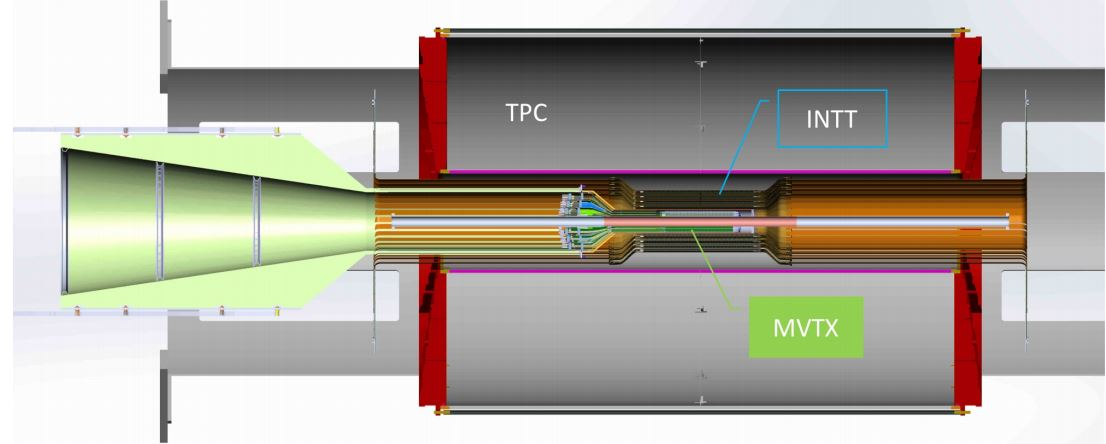
\includegraphics[width=16cm]{assets/mvtx.JPG}
    \caption{ Figura mostrando no detalhe a posição onde o MVTX será instalado. A figura também mostra o experimento sPHENIX e os seus vários sistemas.}
    \label{mvtx}
\end{figure}

%%%mechanica do detector
Como mostra a Fig. \ref{mvtxdetail}.a, cada suporte do MVTX, denominado \textit{stave}, será instrumentalizado com uma fileira de chips com pixelados, que serão colados na placa de refrigeração, e conectados ao circuíto impresso flexível de leitura dos sinais por meio de uma solda de ligação. Como mostra a Fig. \ref{mvtxdetail}.b uma conexão mecânica permitirá que o suporte com os chips sejam conectados ao \textit{end wheel} de onde uma extensão do circuito flexível segue para o \textit{patch panel}, Fig. \ref{mvtxdetail}.c, onde as conexões elétricas são feitas, e onde estão localizados também os serviços de refrigeração e alimentação de baixa tensão dos sensores.

\begin{figure} 
    \centering
    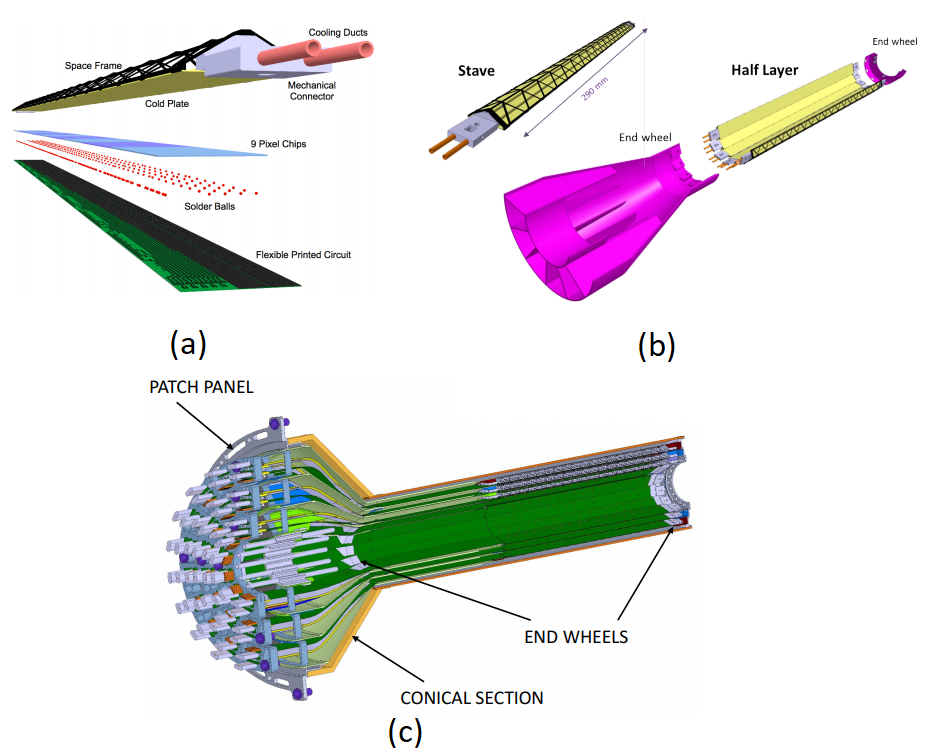
\includegraphics[width=16.0cm]{assets/mvtx_detail.JPG}
    \caption{Figura mostrando detalhes do detector MVTX: (a) Vista esquemática de uma \textit{stave} do MVTX. (b) MVTX \textit{stave}, e conjunto de \textit{staves} fixadas em um suporte formando a metade de um barril do detector. (c) Vista da metade do detector MVTX montado com três camadas fixadas no \textit{end wheel} onde estão localizados os serviços responsáveis por garantir o funcionamento dos sensores.}
    \label{mvtxdetail}
\end{figure}

\renewcommand{\cleardoublepage}{}
\renewcommand{\clearpage}{}